%%%%%%%%%%%%%%%%%%%%%%%%%%%%%%%%%%%%%%%%%
% Thin Sectioned Essay
% LaTeX Template
% Version 1.0 (3/8/13)
%
% This template has been downloaded from:
% http://www.LaTeXTemplates.com
%
% Original Author:
% Nicolas Diaz (nsdiaz@uc.cl) with extensive modifications by:
% Vel (vel@latextemplates.com)
%
% License:
% CC BY-NC-SA 3.0 (http://creativecommons.org/licenses/by-nc-sa/3.0/)
%
%%%%%%%%%%%%%%%%%%%%%%%%%%%%%%%%%%%%%%%%%

%----------------------------------------------------------------------------------------
%	PACKAGES AND OTHER DOCUMENT CONFIGURATIONS
%----------------------------------------------------------------------------------------
\documentclass[12pt]{article} % Font size (can be 10pt, 11pt or 12pt) and paper size (remove a4paper for US letter paper)
\usepackage[protrusion=true,expansion=true]{microtype} % Better typography
\usepackage[left=1in,right=1in,top=.95in,bottom=.95in]{geometry}
\usepackage{graphicx} % Required for including pictures
\usepackage{wrapfig} % Allows in-line images
%\usepackage{mathpazo} % Use the Palatino font
\usepackage[T1]{fontenc} % Required for accented characters
%\linespread{1.05} % Change line spacing here, Palatino benefits from a slight increase by default
%\usepackage{array}
%\usepackage{booktabs}
%\usepackage{latexsym}
\usepackage{fancyhdr}
\usepackage{lastpage}
\usepackage[pdftex]{hyperref}
\usepackage{tipa}
\usepackage{url}
\usepackage{verbatim}
\hypersetup{
  colorlinks = true,
  urlcolor = black,
  citecolor=black,%
  filecolor=black,%
  linkcolor=black,%
  urlcolor=black     % can put red here to visualize the links
}
%\usepackage{biblatex}

\usepackage{outlines}
\usepackage{enumitem}
\usepackage{mathtools}
\usepackage{vector}
\usepackage{fixltx2e}

\usepackage{pdfpages}

\usepackage{xfrac}

\usepackage[labelfont=bf]{caption}

%\usepackage[latin1]{inputenc}
\usepackage{tikz}
\usetikzlibrary{shapes,arrows}


\newcounter{cenum}
\newcounter{cenumsaved}
\setcounter{cenumsaved}{0}
\newcommand{\labelcenum}{\arabic{cenum}.}
\newenvironment{cenumerate}%
{\begin{list}{\labelcenum}{\usecounter{cenum}}%
\setcounter{cenum}{\value{cenumsaved}}}%
{\setcounter{cenumsaved}{\value{cenum}}%
\end{list}}

\renewcommand{\outlineii}{cenumerate}

%\setenumerate[1]{label=\Roman*.}
%\setenumerate[2]{label=\Alph*.}
%\setenumerate[3]{label=\roman*.}
%\setenumerate[4]{label=\alph*.}

\makeatletter
%\renewcommand\@biblabel[1]{\textbf{#1.}} % Change the square brackets for each bibliography item from '[1]' to '1.'
\renewcommand{\@listI}{\itemsep=0pt} % Reduce the space between items in the itemize and enumerate environments and the bibliography

\renewcommand{\maketitle}{ % Customize the title - do not edit title and author name here, see the TITLE block below
\begin{center} % Right align
{\noindent\@title} % Increase the font size of the title

\vspace{10pt} % Some vertical space between the title and author name

{\noindent\@author}\\\@date

\vspace{10pt} % Some vertical space between the author block and abstract
\end{center}
}


\let\oldhat\hat
\renewcommand{\vec}[1]{\mathbf{#1}}
\renewcommand{\hat}[1]{\oldhat{\mathbf{#1}}}


\providecommand{\e}[1]{\ensuremath{\times 10^{#1}}}

%----------------------------------------------------------------------------------------
%	TITLE
%----------------------------------------------------------------------------------------
%\title{\LARGE{\textbf{Software Engineering Best Practices\\in Biomedical Informatics}\\[.5em]
%}}
%
%\author{\large{Nicholas J. Matiasz}\vspace{.4em}}
%
%\date{\large{2013-10-31}} % Date
%----------------------------------------------------------------------------------------

%----------------------------------------------------------------------------------------
%	HEADER/FOOTER
%----------------------------------------------------------------------------------------
\lhead{}
\chead{}
\rhead{}
\lfoot{BE 224A \textpipe\ Ultrasound Lecture}
\cfoot{\thepage\ of\ \pageref{LastPage}}
\rfoot{Nicholas J. Matiasz}
\renewcommand{\headrulewidth}{0.4pt}
\renewcommand{\footrulewidth}{0.4pt}
\pagestyle{fancyplain}



%----------------------------------------------------------------------------------------
%	ESSAY BODY
%----------------------------------------------------------------------------------------
\begin{document}

\begin{titlepage}

\newcommand{\HRule}{\rule{\linewidth}{0.5mm}} % Defines a new command for the horizontal lines, change thickness here

\center % Center everything on the page
 
%----------------------------------------------------------------------------------------
%	HEADING SECTIONS
%----------------------------------------------------------------------------------------

\textsc{\Large University of California, Los Angeles}\\[1.5cm] % Name of your university/college
\textsc{\large Medical Imaging Informatics Group}\\[0.5cm] % Major heading such as course name
\textsc{\large BE 224A Ultrasound Lecture}\\[0.5cm] % Minor heading such as course title

%----------------------------------------------------------------------------------------
%	TITLE SECTION
%----------------------------------------------------------------------------------------
\vspace{20pt}
\HRule \\[0.5cm]
\LARGE{\textbf{Lecture notes on}}\\[.3cm]
\LARGE{\textbf{ultrasound tissue characterization}}\\
\HRule \\[1.5cm]
 
%----------------------------------------------------------------------------------------
%	AUTHOR SECTION
%----------------------------------------------------------------------------------------

\begin{minipage}{0.4\textwidth}
\begin{flushleft} \large
\emph{Author:}\\
Nicholas J.\ Matiasz % Your name
\end{flushleft}
\end{minipage}
~
\begin{minipage}{0.4\textwidth}
\begin{flushright} \large
\emph{Instructor:} \\
Prof.\ Ricky Taira % Supervisor's Name
\end{flushright}
\end{minipage}\\[4cm]

% If you don't want a supervisor, uncomment the two lines below and remove the section above
%\Large \emph{Author:}\\
%John \textsc{Smith}\\[3cm] % Your name

%----------------------------------------------------------------------------------------
%	DATE SECTION
%----------------------------------------------------------------------------------------
\begin{minipage}{0.4\textwidth}
\begin{center} \large
\emph{Submitted:} \\
2014-02-18 % Supervisor's Name
\end{center}
\end{minipage}\\[4cm]
%{\large Submitted: 2013-10-30}\\[3cm] % Date, change the \today to a set date if you want to be precise

%----------------------------------------------------------------------------------------
%	LOGO SECTION
%----------------------------------------------------------------------------------------
%\includegraphics{Logo}\\[1cm] % Include a department/university logo - this will require the graphicx package
%----------------------------------------------------------------------------------------
\vfill % Fill the rest of the page with whitespace
\end{titlepage}


\fontsize{12}{19.416407865}%22.5, 28
\selectfont
%\thispagestyle{empty}
%\tableofcontents

\section{Introduction}
This text is a collection of lecture notes to explain tissue characterization using ultrasound imaging in the clinical setting.



\section{Noise}
Rayleigh distribution: speckle noise in ultrasound images follows this distribution



\section{Summary}


\begin{equation}
c = \lambda f
\label{eq:speed_wavelength_frequency}
\end{equation}

\begin{equation}
c = \sqrt{\frac{\mathrm{B}}{\rho}}
\label{eq:speed_modulus_density}
\end{equation}

\begin{equation}
\mathrm{I} \propto \mathrm{P}^{2}
\label{eq:intensity_pressure}
\end{equation}

\begin{equation}
\text{Relative intensity (dB)} = 10\log\left(\frac{\mathrm{I_2}}{\mathrm{I_1}}\right)
\label{eq:relative_intensity}
\end{equation}

\begin{equation}
\text{Relative pressure (dB)} = 20\log\left(\frac{\mathrm{P_2}}{\mathrm{P_1}}\right)
\label{eq:relative_pressure}
\end{equation}

\begin{equation}
\mathrm{Z} = \rho c
\label{eq:acoustic_impedance}
\end{equation}

\begin{equation}
\mathrm{R_P} = \frac{\mathrm{P_r}}{\mathrm{P_i}} = \frac{\mathrm{\mathrm{Z_2}}-\mathrm{Z_1}}{{\mathrm{Z_2}}+\mathrm{Z_1}}
\label{eq:reflection_pressure_coefficient}
\end{equation}

\begin{equation}
\mathrm{R_I} = \frac{\mathrm{I_r}}{\mathrm{I_i}} = {\left(\frac{\mathrm{\mathrm{Z_2}}-\mathrm{Z_1}}{{\mathrm{Z_2}}+\mathrm{Z_1}}\right)}^{2}
\label{eq:reflection_intensity_coefficient}
\end{equation}

\begin{equation}
\frac{\sin\theta_{\mathrm{t}}}{\sin\theta_{\mathrm{i}}} = \frac{c_{2}}{c_{1}}
\label{eq:snells_law}
\end{equation}

\begin{equation}
\frac{\theta_{\mathrm{t}}}{\theta_{\mathrm{i}}} \cong \frac{c_{2}}{c_{1}}
\label{eq:snells_law_approximation}
\end{equation}

\begin{equation}
\theta_{\mathrm{c}} = \arcsin\left(\frac{c_{1}}{c_{2}}\right)
\label{eq:snells_law_critical_angle}
\end{equation}

\begin{equation}
\mathrm{Q} = \frac{f_{0}}{\mathrm{Bandwidth}}
\label{eq:q_factor}
\end{equation}

\begin{equation}
\mathrm{Q} = \frac{f_{0}}{\mathrm{Bandwidth}}
\label{eq:near_field_length}
\end{equation}

%\begin{equation}
%\frac{N_{2}}{N_{1}} = e^{-\frac{\Delta E}{kT}}
%\label{eq:spin_up_spin_down}
%\end{equation}

%\begin{figure}[h]
%\centering
%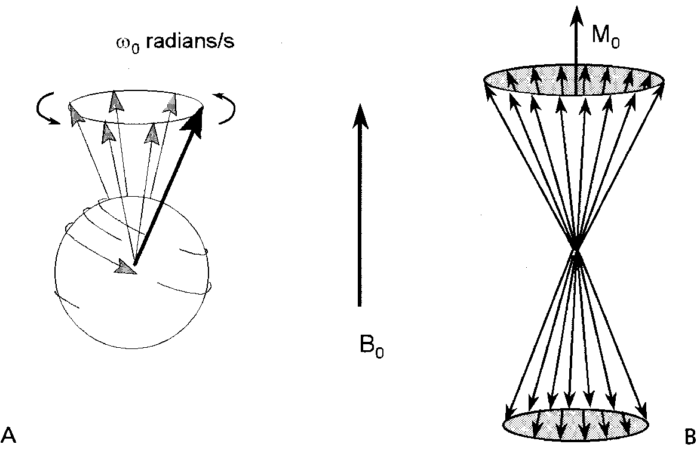
\includegraphics[scale=0.75]{./images/spins_in_b0.png}
%\caption{\textbf{A}: An illustration of the Larmor frequency. \textbf{B}: The net magnetization vector that occurs in the presence of $\vec{B_{0}}$ \cite{bushberg2002}.}
%\label{fig:spins_in_b0}
%\end{figure}


%----------------------------------------------------------------------------------------
%	BIBLIOGRAPHY
%----------------------------------------------------------------------------------------
%\newpage
\bibliographystyle{plain}
\bibliography{224a_ultrasound_lecture}
%----------------------------------------------------------------------------------------

\end{document}